\newpage
\section{Results Analysis}
\label{sec:results}

In this section, we first present the runs that achieved the highest and lowest scores on the train and test data.
Subsequently, we provide an interpretation and analysis of these score values (see Section~\ref{subsec:discussion}).

\subsection{Training Data and Selection of Runs to Submit}\label{subsec:runs_selection}

\begin{table}[h!]
    \begin{center}
        \caption{MAP and NCDG scores for all the runs on the training collection}
        \label{tab:all_scores}
        \begin{tabular}{|c|c||c|c|}
            \hline
            \textbf{Run ID} & \textbf{Run} & \textbf{MAP Score} & \textbf{NCDG Score}\\
            \hline\hline
            01 & en\_en & \cellcolor{red!30!white}0.0700 & \cellcolor{red!30!white}0.1614 \\
            \hline
            02 & en\_en\_3gram & 0.0704 & 0.1661 \\
            \hline
            03 & en\_en\_4gram & 0.0874 & 0.2025 \\
            \hline
            04 & en\_en\_5gram & 0.1028 & 0.2288 \\
            \hline
            05 & en\_en\_fr\_5gram & \cellcolor{red!60!white}0.0669 & \cellcolor{red!60!white}0.1525 \\
            \hline
            06 & en\_en\_4gram\_ner & \cellcolor{red}0.0360 & \cellcolor{red}0.1098 \\
            \hline
            07 & fr\_fr & 0.1656 & 0.3135 \\
            \hline
            08 & fr\_fr\_3gram & \cellcolor{green!30!white}0.1698 & \cellcolor{green!30!white}0.3208 \\
            \hline
            09 & fr\_fr\_4gram & \cellcolor{green!60!white}0.1737 & \cellcolor{green!60!white}0.3269 \\
            \hline
            10 & fr\_fr\_5gram & \cellcolor{green}0.1748 & \cellcolor{green}0.3285 \\
            \hline
            11 & fr\_en\_fr\_5gram & 0.1288 & 0.2797 \\
            \hline
            12 & fr\_fr\_4gram\_ner & 0.1362 & 0.2881 \\
            \hline
        \end{tabular}
    \end{center}
\end{table}

% Ferro said that with this data we should only use the tables
%\begin{figure}[h!]
%    \centering
%    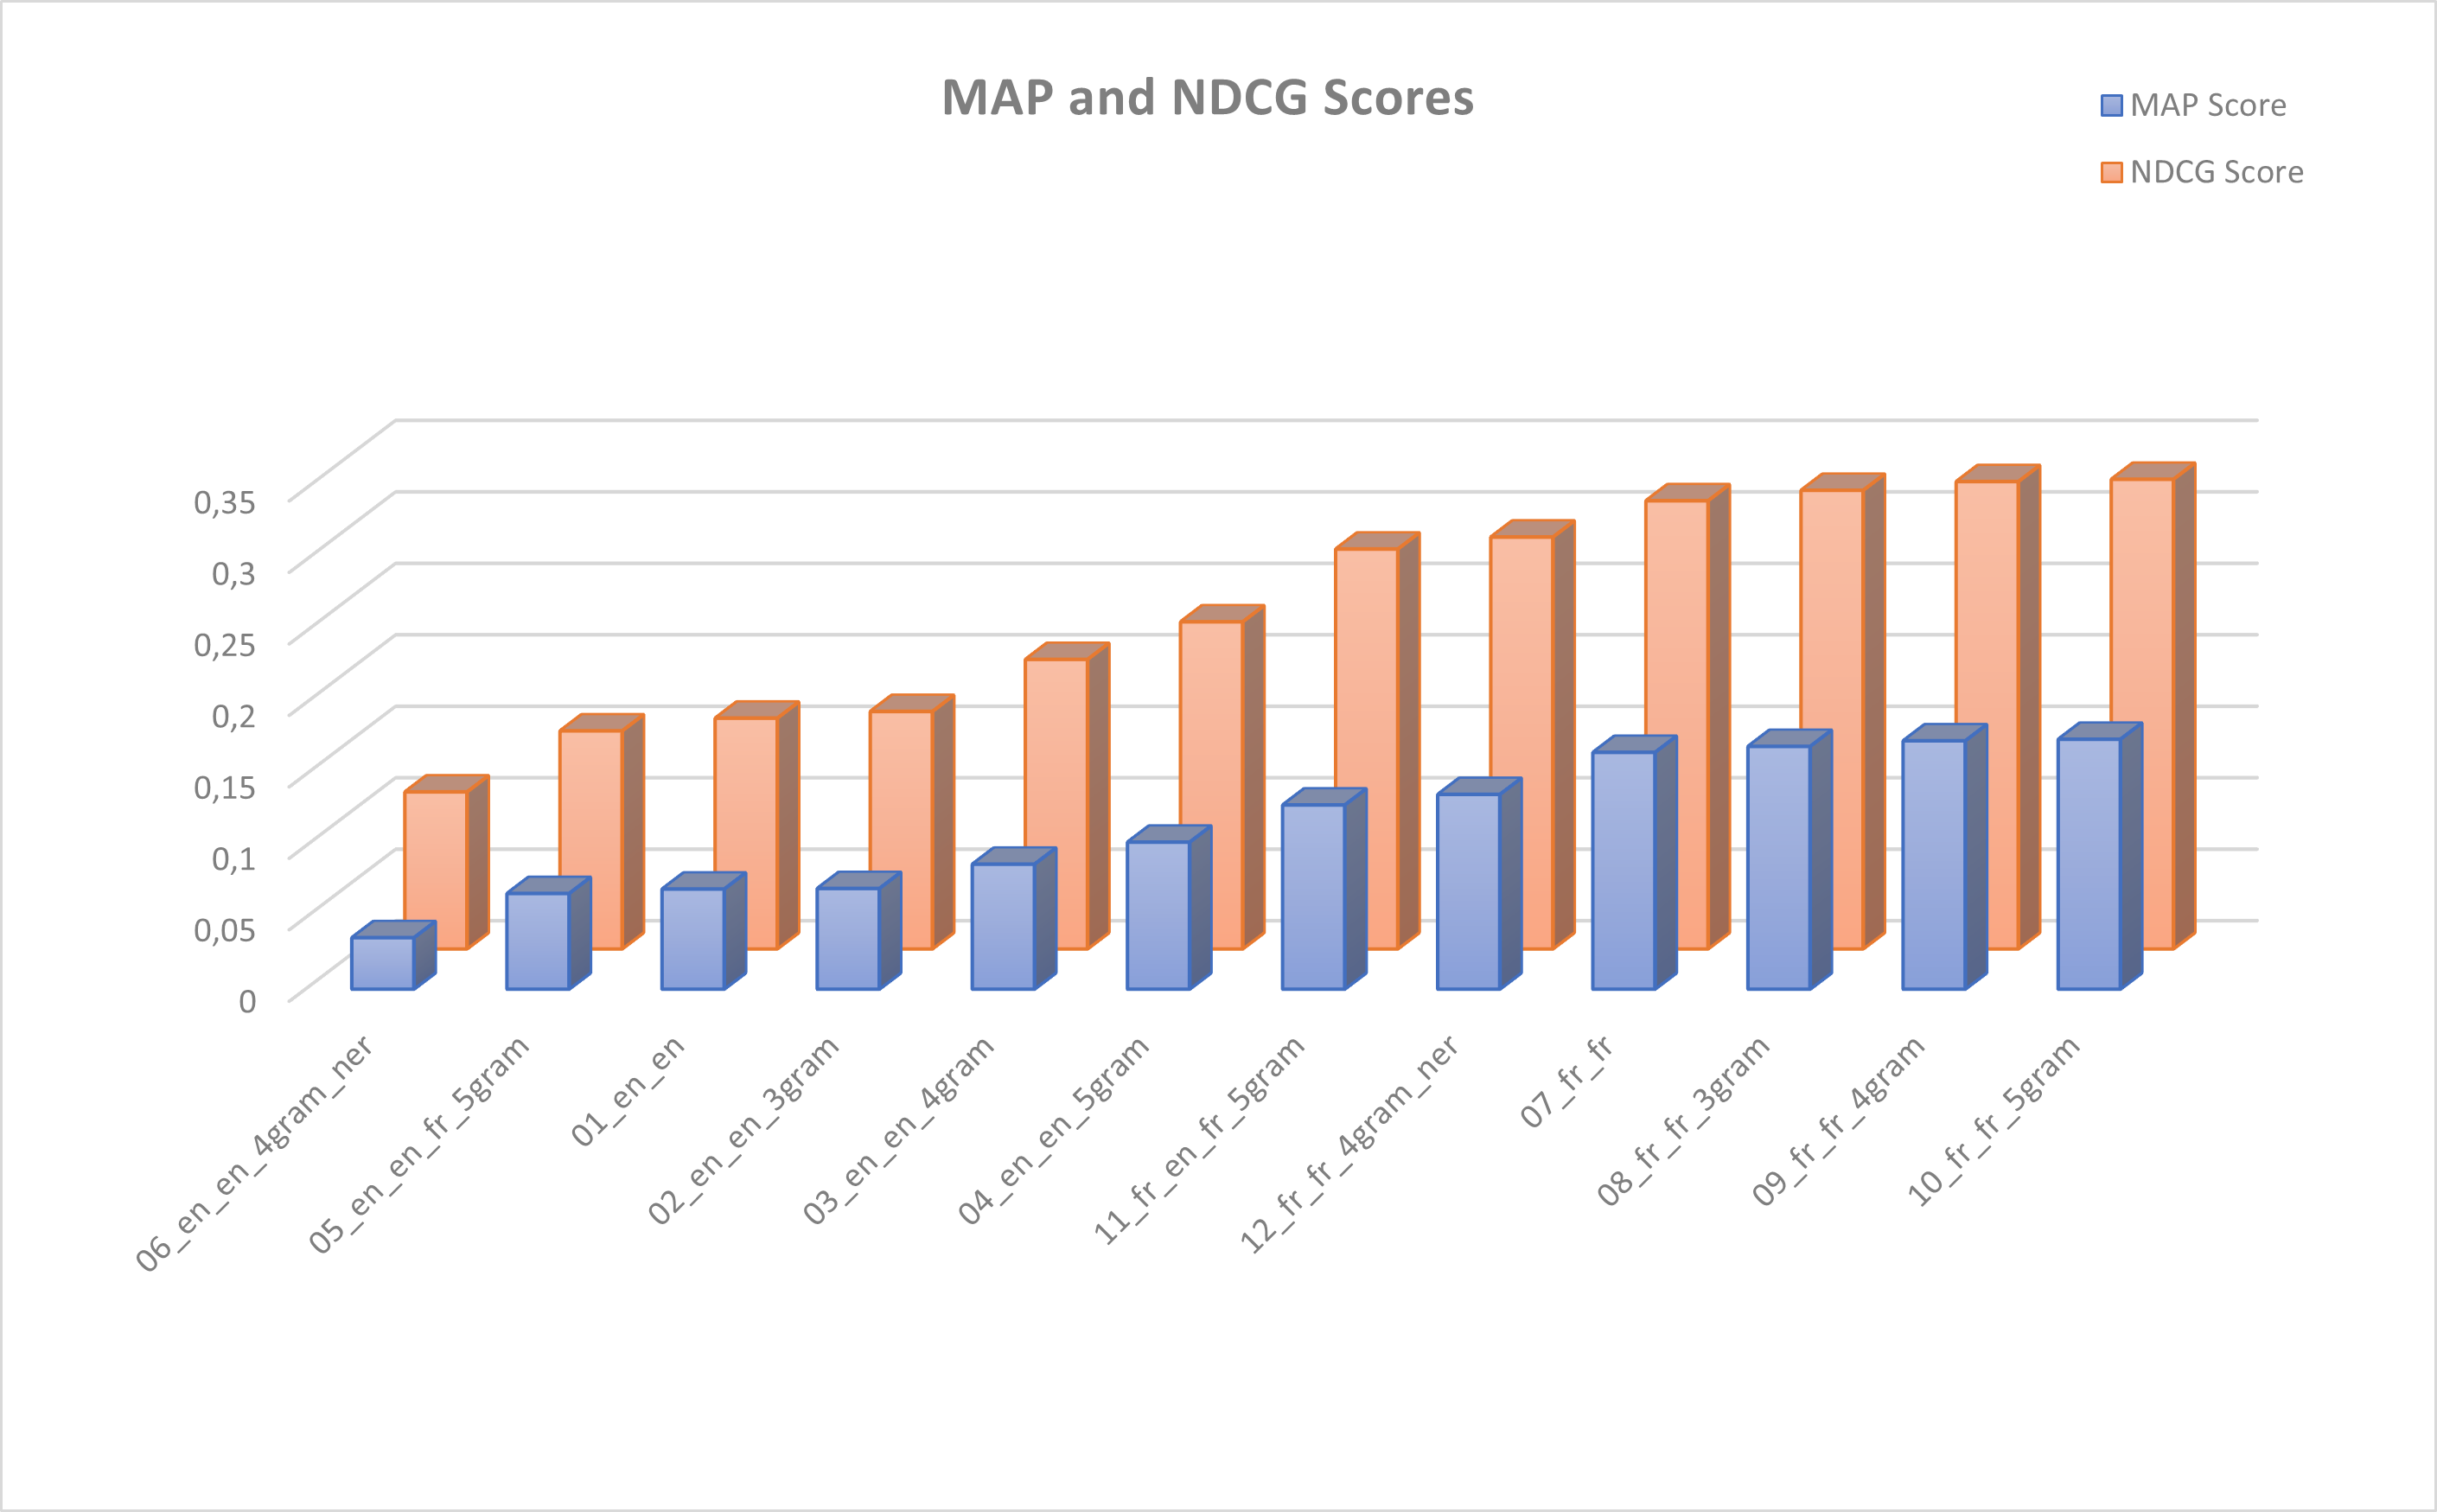
\includegraphics[width=0.6\textwidth]{figure/allScores}
%    \caption{All scores sorted by MAP score}
%    \label{fig:sorted_scores}
%\end{figure}

The analysis shows that, on training data, the highest MAP score (0.1748) is achieved by \texttt{10\_fr\_fr\_5gram},
followed by
\texttt{09\_fr\_fr\_4gram} (0.1737),
\texttt{08\_fr\_fr\_3gram} (0.1698),
\texttt{07\_fr\_fr} (0.1656), and
\texttt{12\_fr\_fr\_4gram\_ner} (0.1362).
The lowest MAP score (0.0360) is obtained by \texttt{en\_en\_4gram\_ner}.\\

Similarly, the highest NDCG score (0.3285) belongs to \texttt{10\_fr\_fr\_5gram}, followed by
\texttt{09\_fr\_fr\_4gram} (0.3269),
\texttt{08\_fr\_fr\_3gram} (0.3208),
\texttt{07\_fr\_fr} (0.3135), and
\texttt{12\_fr\_fr\_4gram\_ner} (0.2881).
The lowest NDCG score (0.1098) corresponds to \texttt{en\_en\_4gram\_ner}.\\

Because of this, the five system submitted to CLEF have been (in order of importance): \texttt{10\_fr\_fr\_5gram},
\texttt{09\_fr\_fr\_4gram}, \texttt{08\_fr\_fr\_3gram}, \texttt{07\_fr\_fr}, and \texttt{12\_fr\_fr\_4gram\_ner}.
Following the competition workflow, we created new indexes based on the test collection and re-executed this top five
runs.\\

% Ferro said that with this data we should only use the tables
%Here we can see a chart ranking of the five best scores, they are the runs that have been presented at CLEF:
%\begin{figure}[h!]
%    \centering
%    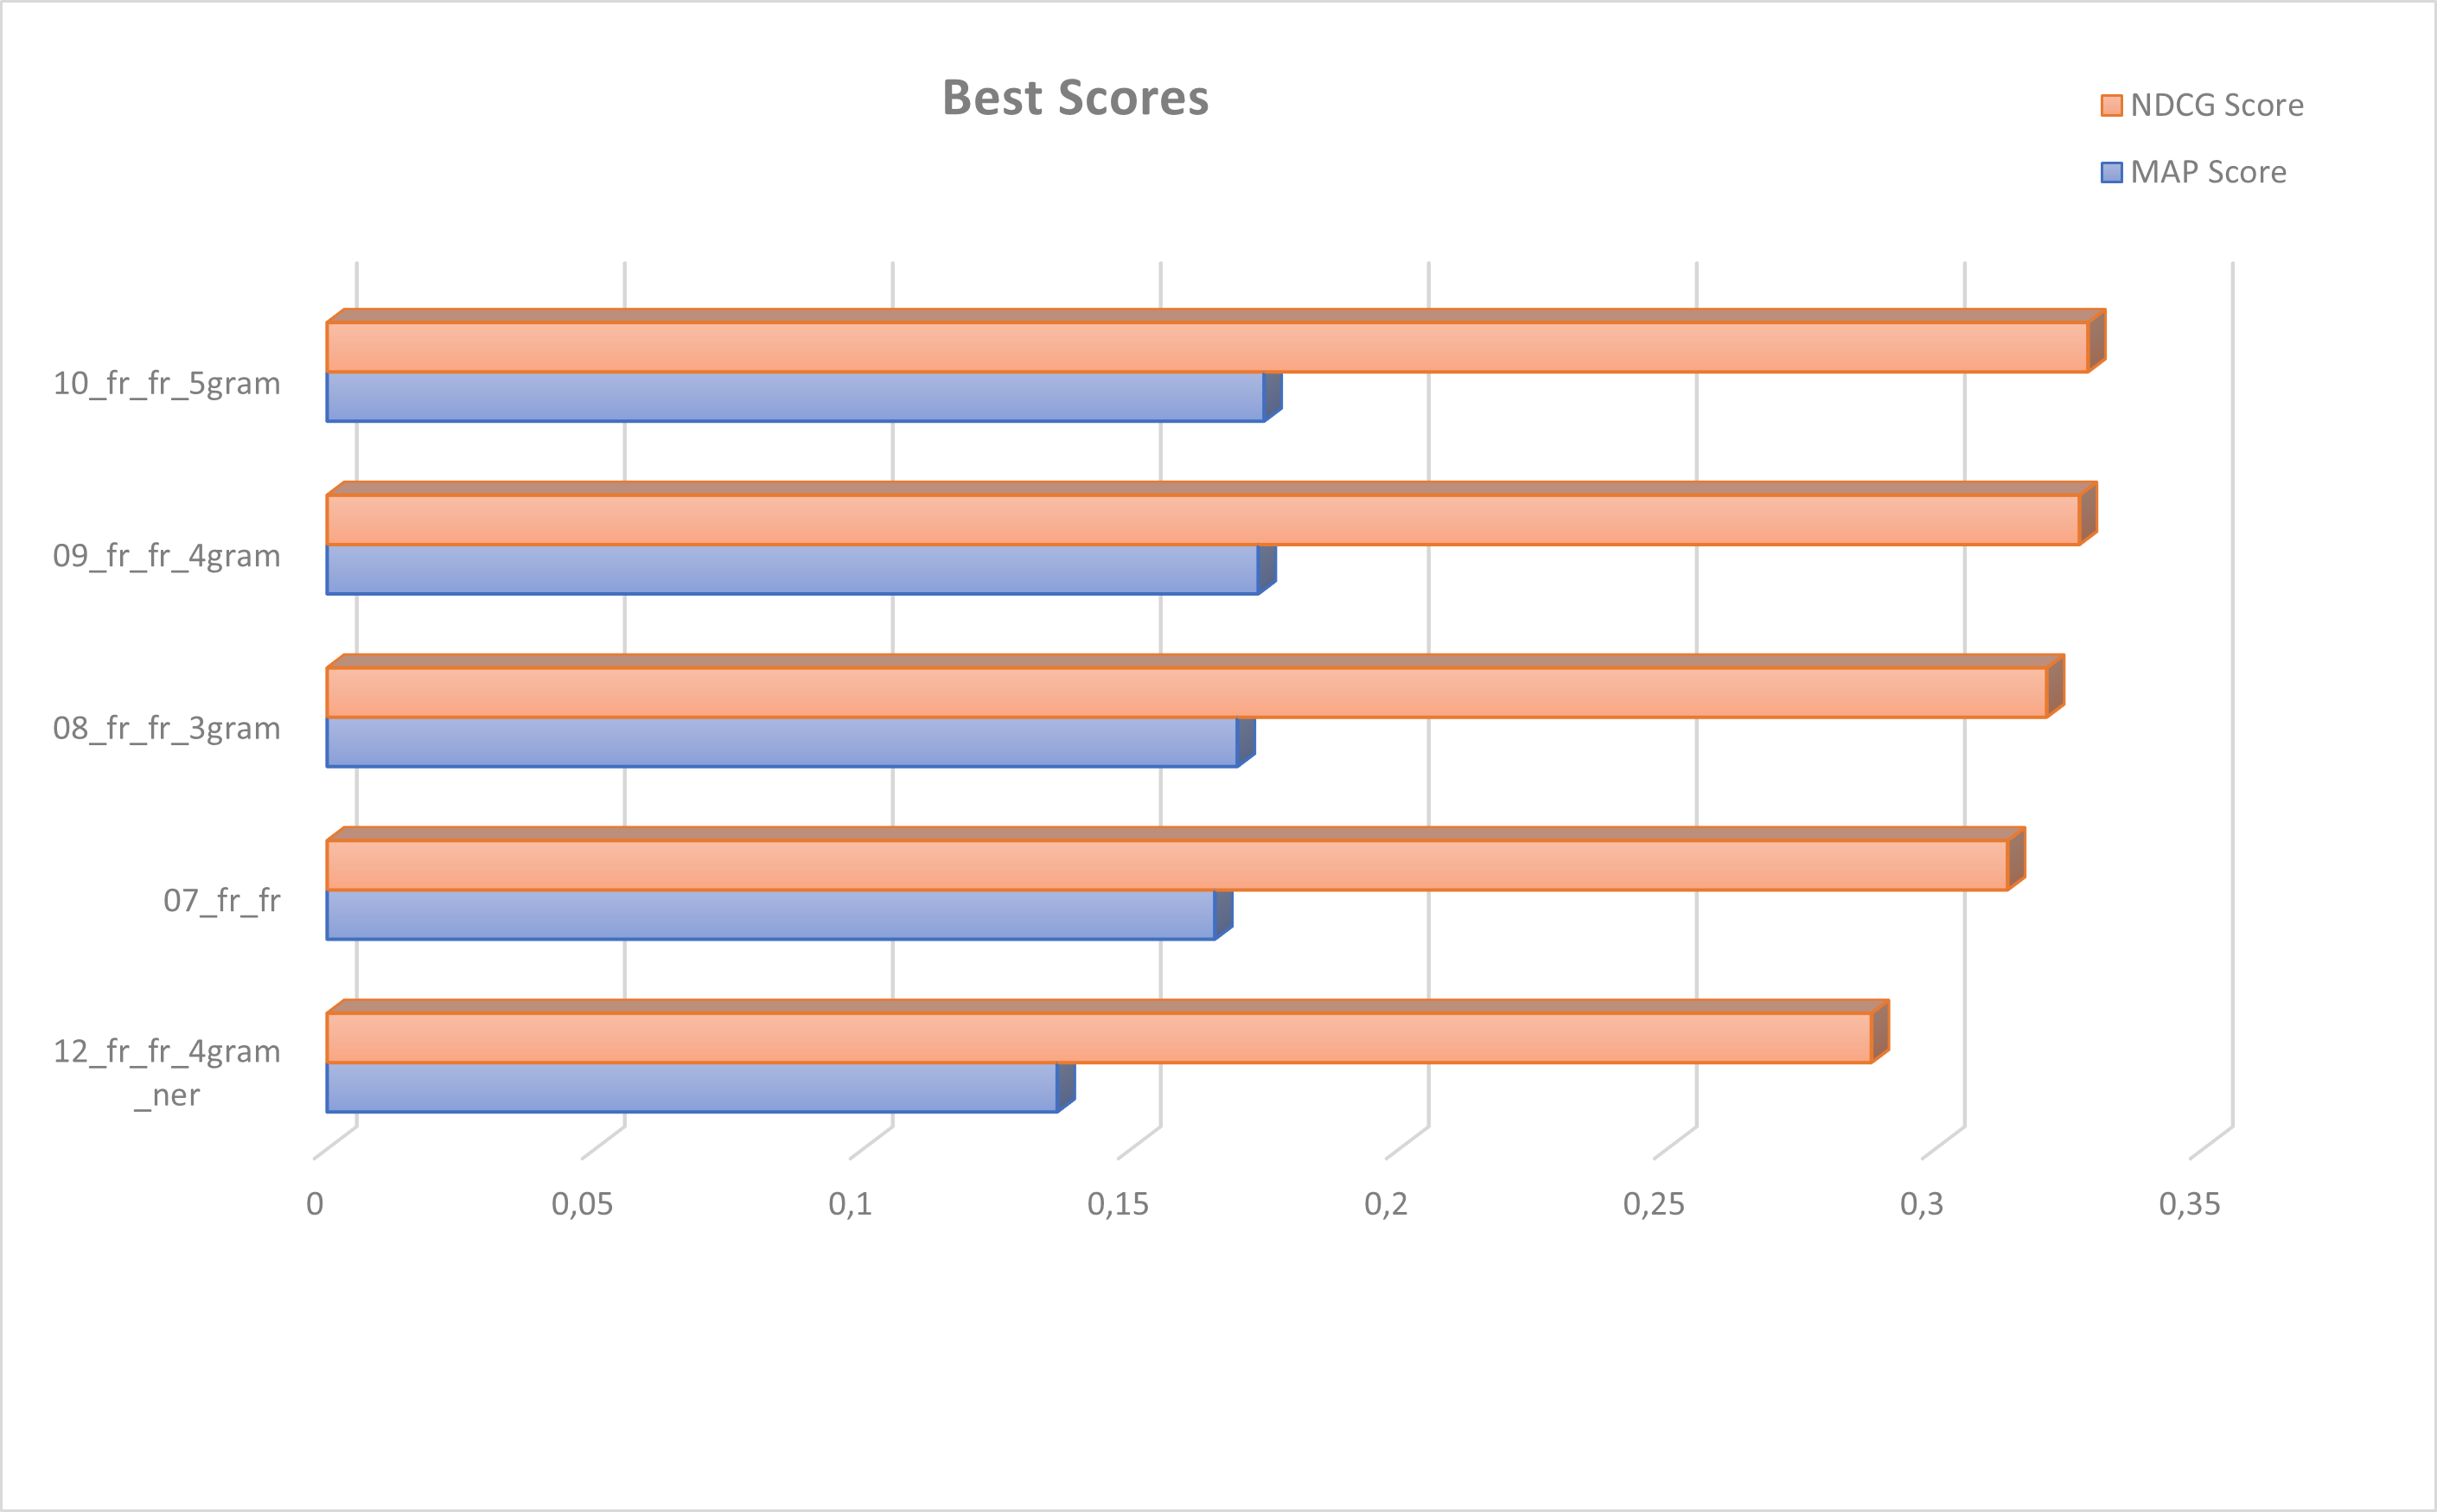
\includegraphics[width=0.6\textwidth]{figure/bestScores}
%    \caption{Best MAP and NDCG scores}
%    \label{fig:best_scores}
%\end{figure}

\subsection{Short Term Test Data}\label{subsec:short_term}

Table~\ref{tab:st_scores} presents the mentioned scores computed for our five submitted systems on the (test)
short-term collection.\\

% Very interesting: https://www.reneshbedre.com/blog/anova.html
In the Two-Way ANOVA analysis presented in Table~\ref{tab:st_anova} we observed a significant p-value (p < 0.05).
Thus, we can conclude that there are significant differences among our systems.
As ANOVA does not tell which systems are significantly different from each other, in Table~\ref{tab:st_comparison} we
can observe the Tukey’s Honestly Significantly Differenced (HSD) test.
It suggests that pairwise comparisons between systems 7--12, 8--12, 9--12 and 10--12 reject null hypothesis (p < 0.05)
and indicate statistical significant differences.

\begin{table}[h!]
    \begin{center}
        \caption{MAP, NCDG and Rprec scores for the submitted runs on the (test) short-term collection}
        \label{tab:st_scores}
        \begin{tabular}{|c|c||c|c|c|}
            \hline
            \textbf{Run ID} & \textbf{Run} & \textbf{NCDG Score} & \textbf{MAP Score} & \textbf{RPREC Score}\\
            \hline\hline
            07 & fr\_fr & 0.3367 & 0.1883 & 0.1561 \\
            \hline
            08 & fr\_fr\_3gram & 0.3384 & 0.1893 & 0.1579 \\
            \hline
            09 & fr\_fr\_4gram & 0.3423 & 0.1911 & 0.1581 \\
            \hline
            10 & fr\_fr\_5gram & 0.3447 & 0.1926 & 0.1603 \\
            \hline
            12 & fr\_fr\_4gram\_ner & 0.2980 & 0.1468 & 0.1172 \\
            \hline
        \end{tabular}
    \end{center}
\end{table}

\begin{table}[h!]
    \centering
    \caption{Two-Way ANOVA table assessing AP for the submitted systems on the (test) short-term collection}
    \label{tab:st_anova}
    \begin{tabular}{|l|l|l|l|l|l|}
    \hline
        \textbf{Source} & \textbf{DF} & \textbf{SS} & \textbf{MS} & \textbf{F} & \textbf{PR(>F)} \\ \hline\hline
        \textbf{C(system)} & 4 & 1.348254 & 0.337063 & 6.250613 & 0.000052 \\ \hline
        \textbf{Error} & 4405 & 237.539013 & 0.053925 & -- & -- \\ \hline
        \textbf{Total} & 4409 & 238.887267 & -- & -- & -- \\ \hline
    \end{tabular}
\end{table}

\begin{table}[h!]
    \centering
    \caption{Tukey Honestly Significant Difference test for the submitted systems on the (test) short-term collection}
    \label{tab:st_comparison}
    \begin{tabular}{|l|l||c|c|c|c|c|}
        \hline
        \textbf{Run 1} & \textbf{Run 2} & \textbf{Diff} & \textbf{Lower} & \textbf{Upper} & \textbf{q-value} & \textbf{p-value} \\ \hline\hline
        07\_fr\_fr & 08\_fr\_fr\_3gram & 0.000986 & -0.029190 & 0.031162 & 0.126122 & 0.900000 \\ \hline
        07\_fr\_fr & 09\_fr\_fr\_4gram & 0.002808 & -0.027368 & 0.032984 & 0.359124 & 0.900000 \\ \hline
        07\_fr\_fr & 10\_fr\_fr\_5gram & 0.004282 & -0.025894 & 0.034458 & 0.547611 & 0.900000 \\ \hline
        07\_fr\_fr & 12\_fr\_fr\_4gram\_ner & 0.041538 & 0.011362 & 0.071714 & 5.312288 & 0.001641 \\ \hline
        08\_fr\_fr\_3gram & 09\_fr\_fr\_4gram & 0.001822 & -0.028354 & 0.031998 & 0.233002 & 0.900000 \\ \hline
        08\_fr\_fr\_3gram & 10\_fr\_fr\_5gram & 0.003296 & -0.026880 & 0.033472 & 0.421489 & 0.900000 \\ \hline
        08\_fr\_fr\_3gram & 12\_fr\_fr\_4gram\_ner & 0.042524 & 0.012348 & 0.072700 & 5.438410 & 0.001152 \\ \hline
        09\_fr\_fr\_4gram & 10\_fr\_fr\_5gram & 0.001474 & -0.028702 & 0.031650 & 0.188487 & 0.900000 \\ \hline
        09\_fr\_fr\_4gram & 12\_fr\_fr\_4gram\_ner & 0.044346 & 0.014170 & 0.074522 & 5.671412 & 0.001000 \\ \hline
        10\_fr\_fr\_5gram & 12\_fr\_fr\_4gram\_ner & 0.045820 & 0.015644 & 0.075995 & 5.859899 & 0.001000 \\ \hline
    \end{tabular}
\end{table}

\subsection{Long Term Test Data}\label{subsec:long_term}

Table~\ref{tab:lt_scores} presents the mentioned scores computed for our five submitted systems on the (test)
long-term collection.\\

In the Two-Way ANOVA analysis presented in Table~\ref{tab:lt_anova} we observed a significant p-value (p < 0.05), so we
can conclude that there are significant differences among our systems.
The Tukey's Honestly Significantly Differenced (HSD) test in Table~\ref{tab:lt_comparison} again suggests that pairwise
comparisons between systems 7--12, 8--12, 9--12 and 10--12 reject null hypothesis (p < 0.05).

\begin{table}[h!]
    \begin{center}
        \caption{MAP, NCDG and Rprec scores for the submitted runs on the (test) long-term collection}
        \label{tab:lt_scores}
        \begin{tabular}{|c|c||c|c|c|}
            \hline
            \textbf{Run ID} & \textbf{Run} & \textbf{NCDG Score} & \textbf{MAP Score} & \textbf{RPREC Score}\\
            \hline\hline
            07 & fr\_fr & 0.3447 & 0.1880 & 0.1589 \\
            \hline
            08 & fr\_fr\_3gram & 0.3454 & 0.1881 & 0.1600 \\
            \hline
            09 & fr\_fr\_4gram & 0.3480 & 0.1888 & 0.1611 \\
            \hline
            10 & fr\_fr\_5gram & 0.3533 & 0.1920 & 0.1642 \\
            \hline
            12 & fr\_fr\_4gram\_ner & 0.3046 & 0.1433 & 0.1192\\
            \hline
        \end{tabular}
    \end{center}
\end{table}

\begin{table}[!ht]
    \centering
    \caption{Two-Way ANOVA table assessing AP for the submitted systems on the (test) long-term collection}
    \label{tab:lt_anova}
    \begin{tabular}{|l|l|l|l|l|l|}
    \hline
        \textbf{Source} & \textbf{DF} & \textbf{SS} & \textbf{MS} & \textbf{F} & \textbf{PR(>F)} \\ \hline\hline
        \textbf{C(system)} & 4 & 1.564386 & 0.391097 & 8.562506 & 7.01E-07 \\ \hline
        \textbf{Error} & 4610 & 210.56392 & 0.045675 & -- & -- \\ \hline
        \textbf{Total} & 4614 & 212.128306 & -- & -- & -- \\ \hline
    \end{tabular}
\end{table}

\begin{table}[h!]
    \centering
    \caption{Tukey Honestly Significant Difference test for the submitted systems on the (test) long-term collection}
    \label{tab:lt_comparison}
    \begin{tabular}{|l|l||c|c|c|c|c|}
        \hline
        \textbf{Run 1} & \textbf{Run 2} & \textbf{Diff} & \textbf{Lower} & \textbf{Upper} & \textbf{q-value} & \textbf{p-value} \\ \hline\hline
        07\_fr\_fr & 08\_fr\_fr\_3gram & 0.000340 & -0.026808 & 0.027488 & 0.048345 & 0.900000 \\ \hline
        07\_fr\_fr & 09\_fr\_fr\_4gram & 0.001090 & -0.026058 & 0.028237 & 0.154891 & 0.900000 \\ \hline
        07\_fr\_fr & 10\_fr\_fr\_5gram & 0.004239 & -0.022909 & 0.031387 & 0.602592 & 0.900000 \\ \hline
        07\_fr\_fr & 12\_fr\_fr\_4gram\_ner & 0.044458 & 0.017311 & 0.071606 & 6.319943 & 0.001000 \\ \hline
        08\_fr\_fr\_3gram & 09\_fr\_fr\_4gram & 0.000750 & -0.026398 & 0.027897 & 0.106546 & 0.900000 \\ \hline
        08\_fr\_fr\_3gram & 10\_fr\_fr\_5gram & 0.003899 & -0.023249 & 0.031047 & 0.554247 & 0.900000 \\ \hline
        08\_fr\_fr\_3gram & 12\_fr\_fr\_4gram\_ner & 0.044798 & 0.017651 & 0.071946 & 6.368287 & 0.001000 \\ \hline
        09\_fr\_fr\_4gram & 10\_fr\_fr\_5gram & 0.003149 & -0.023998 & 0.030297 & 0.447701 & 0.900000 \\ \hline
        09\_fr\_fr\_4gram & 12\_fr\_fr\_4gram\_ner & 0.045548 & 0.018400 & 0.072696 & 6.474833 & 0.001000 \\ \hline
        10\_fr\_fr\_5gram & 12\_fr\_fr\_4gram\_ner & 0.048697 & 0.021550 & 0.075845 & 6.922534 & 0.001000 \\ \hline
    \end{tabular}
\end{table}

\subsection{Held Out Test Data}\label{subsec:held_out}

Table~\ref{tab:ho_scores} presents mentioned scores computed for our five submitted systems on the (train)
held-out collection.\\

In the Two-Way ANOVA analysis presented in Table~\ref{tab:ho_anova} we didn't observe a significant p-value (p >= 0.05),
so we can conclude that there are not significant differences among our systems.

\begin{table}[h!]
    \begin{center}
        \caption{MAP, NCDG and Rprec scores for the submitted runs on the training collection, held-out evaluation}
        \label{tab:ho_scores}
        \begin{tabular}{|c|c||c|c|c|}
            \hline
            \textbf{Run ID} & \textbf{Run} & \textbf{NCDG Score} & \textbf{MAP Score} & \textbf{RPREC Score}\\
            \hline\hline
            07 & fr\_fr & 0.3271 & 0.1746 & 0.1397 \\
            \hline
            08 & fr\_fr\_3gram & 0.3307 & 0.1725 & 0.1326 \\
            \hline
            09 & fr\_fr\_4gram & 0.3364 & 0.1763 & 0.1397 \\
            \hline
            10 & fr\_fr\_5gram & 0.3413 & 0.1788 & 0.1385 \\
            \hline
            12 & fr\_fr\_4gram\_ner & 0.2868 & 0.1369 & 0.1004 \\
            \hline
        \end{tabular}
    \end{center}
\end{table}

\begin{table}[h!]
    \centering
    \caption{Two-Way ANOVA table assessing AP on the training collection, held-out evaluation}
    \label{tab:ho_anova}
    \begin{tabular}{|l|l|l|l|l|l|}
    \hline
        \textbf{Source} & \textbf{DF} & \textbf{SS} & \textbf{MS} & \textbf{F} & \textbf{PR(>F)} \\ \hline\hline
        \textbf{C(system)} & 4 & 0.11896 & 0.02974 & 0.689161 & 0.599712 \\ \hline
        \textbf{Error} & 485 & 20.929668 & 0.043154 & -- & -- \\ \hline
        \textbf{Total} & 489 & 21.048628 & -- & -- & -- \\ \hline
    \end{tabular}
\end{table}

%\begin{table}[h!]
%    \centering
%    \caption{Other scores}
%    \label{tab:ho_comparison}
%    \begin{tabular}{|r|l|l||c|c|c|c|c|}
%    \hline
%        \multicolumn{8}{|l|}{\textbf{HELD-OUT SECTION}} \\ \hline\hline
%        \textbf{ID} & \textbf{group 1} & \textbf{group 2} & \textbf{Diff} & \textbf{Lower} & \textbf{Upper} & \textbf{q-value} & \textbf{p-value} \\ \hline
%        0 & 07\_fr\_fr & 08\_fr\_fr\_3gram & 0,002054 & -0,079203 & 0,083311 & 0,097886 & 0,900000 \\ \hline
%        1 & 07\_fr\_fr & 09\_fr\_fr\_4gram & 0,001704 & -0,079553 & 0,082961 & 0,081207 & 0,900000 \\ \hline
%        2 & 07\_fr\_fr & 10\_fr\_fr\_5gram & 0,004244 & -0,077013 & 0,085501 & 0,202239 & 0,900000 \\ \hline
%        3 & 07\_fr\_fr & 12\_fr\_fr\_4gram\_ner & 0,037636 & -0,043621 & 0,118892 & 1,793506 & 0,685812 \\ \hline
%        4 & 08\_fr\_fr\_3gram & 09\_fr\_fr\_4gram & 0,003758 & -0,077499 & 0,085015 & 0,179093 & 0,900000 \\ \hline
%        5 & 08\_fr\_fr\_3gram & 10\_fr\_fr\_5gram & 0,006298 & -0,074959 & 0,087555 & 0,300125 & 0,900000 \\ \hline
%        6 & 08\_fr\_fr\_3gram & 12\_fr\_fr\_4gram\_ner & 0,035582 & -0,045675 & 0,116838 & 1,695620 & 0,725010 \\ \hline
%        7 & 09\_fr\_fr\_4gram & 10\_fr\_fr\_5gram & 0,002540 & -0,078717 & 0,083797 & 0,121032 & 0,900000 \\ \hline
%        8 & 09\_fr\_fr\_4gram & 12\_fr\_fr\_4gram\_ner & 0,039340 & -0,041917 & 0,120597 & 1,874713 & 0,653298 \\ \hline
%        9 & 10\_fr\_fr\_5gram & 12\_fr\_fr\_4gram\_ner & 0,041880 & -0,039377 & 0,123136 & 1,995746 & 0,604835 \\ \hline
%    \end{tabular}
%\end{table}

\subsection{Discussion}\label{subsec:discussion}

Results suggest that French queries perform better than their English counterparts, possibly due to the training data's
French origin and later translation into English.
Moreover, the IR system's effectiveness generally increases with a larger N-gram size, as indicated by the higher scores
of \texttt{04\_en\_en\_5gram} and \texttt{10\_fr\_fr\_5gram}.
Conversely, the inclusion of NER in the indexing process seems to have a negative impact on the scores, as shown by the
lower scores of \texttt{06\_en\_en\_4gram\_ner} and \texttt{12\_fr\_fr\_4gram\_ner}.
The use of query expansion with synonyms in English does not seem to improve the search results to any great extent.\\

It's interesting to notice that the cross-language approaches (\texttt{05\_en\_en\_fr\_5gram} and
\texttt{1\_fr\_en\_fr\_5gram}) are out of the five bests systems.
It turns out that searching for English words in French documents and vice versa messes up the search, lowering the
score.
Another interesting aspect is that the worst-performing index is the one with named entity recognition in English
(\texttt{06\_en\_en\_4gram\_ner}): it combines translated queries and NER, which appears to be the two worst-performing
approaches.\\

Our findings indicate that the MAP and NDCG scores in the training data closely align with those in the test data.
Interestingly, there are instances where the scores in the test data show improvement compared to the training data.
Thus, according to the test data, the ranking of our best-performing systems is the same as in
Section~\ref{subsec:runs_selection} (in order of importance): \texttt{10\_fr\_fr\_5gram},
\texttt{09\_fr\_fr\_4gram}, \texttt{08\_fr\_fr\_3gram}, \texttt{07\_fr\_fr}, and \texttt{12\_fr\_fr\_4gram\_ner}.\\

Based on the ANOVA analysis, the null hypothesis is only not rejected in the runs on the held-out collection, suggesting
no statistically significant difference.
We attribute this finding to the limited number of queries in that particular collection.
However, in cases where a statistical significant difference exists among the systems, it appears that system number 12
(\texttt{12\_fr\_fr\_4gram\_ner}) is the only one with a significant impact.
This aligns with our expectations since system number 12 is the only submission utilizing NER among the others.\\

In general, we focused on trying multiple approaches, this is why our score has such a big space for improvement.
As already said, French queries with bigger N-gram sizes perform better.
In this system, instead of relying on single-word matches, the queries take place with more context, resulting in better
search results.\\